%!LW recipe=uplatex

\documentclass[0_main]{subfiles}

\begin{document}

\ifEn
    \section{Quasi-Newton Methods}
\else
    \section{準ニュートン法}
\fi
\label{sec:background_quasi_newton}

\ifEn
    In this section, we discuss quasi-Newton methods. Quasi-Newton methods are based on Newton's method but aim to reduce its primary drawback, namely the high computational cost of evaluating the Hessian matrix. Instead of using the true Hessian matrix $\nabla^2 f(x_k)$, an approximation matrix $B_k$ is employed, thereby achieving fast convergence while keeping the computational cost low.
\else
    本節では準ニュートン法について説明します。準ニュートン法はニュートン法に基づいていますが、その主要な欠点であるヘッセ行列やその逆行列の計算コストを低減することを目的としています。具体的には、真のヘッセ行列 $\nabla^2 f(x_k)$ の代わりに近似行列 $B_k$ とその逆行列 $H_k$ を用いることで、高速な収束性を保ちつつ計算コストを抑えます。
\fi

\ifEn
    \Cref{fig:newton_vs_qs_vs_gd} shows a comparison of Newton's method, quasi-Newton methods, and gradient descent. Gradient descent updates the iterate in the direction opposite to the gradient. Although its per-iteration computational cost is the lowest, its convergence is slow. Newton's method requires the fewest iterations, but it has the highest computational cost per step. Quasi-Newton methods lie between these two extremes and strike a balance between them. In particular, when the methods are compared in terms of total computation time rather than the number of iterations, quasi-Newton methods often exhibit the best performance.
\else
    \Cref{fig:newton_vs_qs_vs_gd} はニュートン法、準ニュートン法、勾配降下法の比較を示しています。勾配降下法は勾配の反対方向に単純に更新する方法です。1反復あたりの計算コストは最小ですが、収束は遅くなります。ニュートン法は反復回数が最も少ない一方で、1ステップあたりの計算コストが最も高いです。準ニュートン法はその中間に位置し、両者のバランスを取っています。特に、反復回数ではなく実際の計算時間で比較すると、準ニュートン法が最良の性能を示すことが多いです。
\fi

\begin{figure}[t]
    \centering
    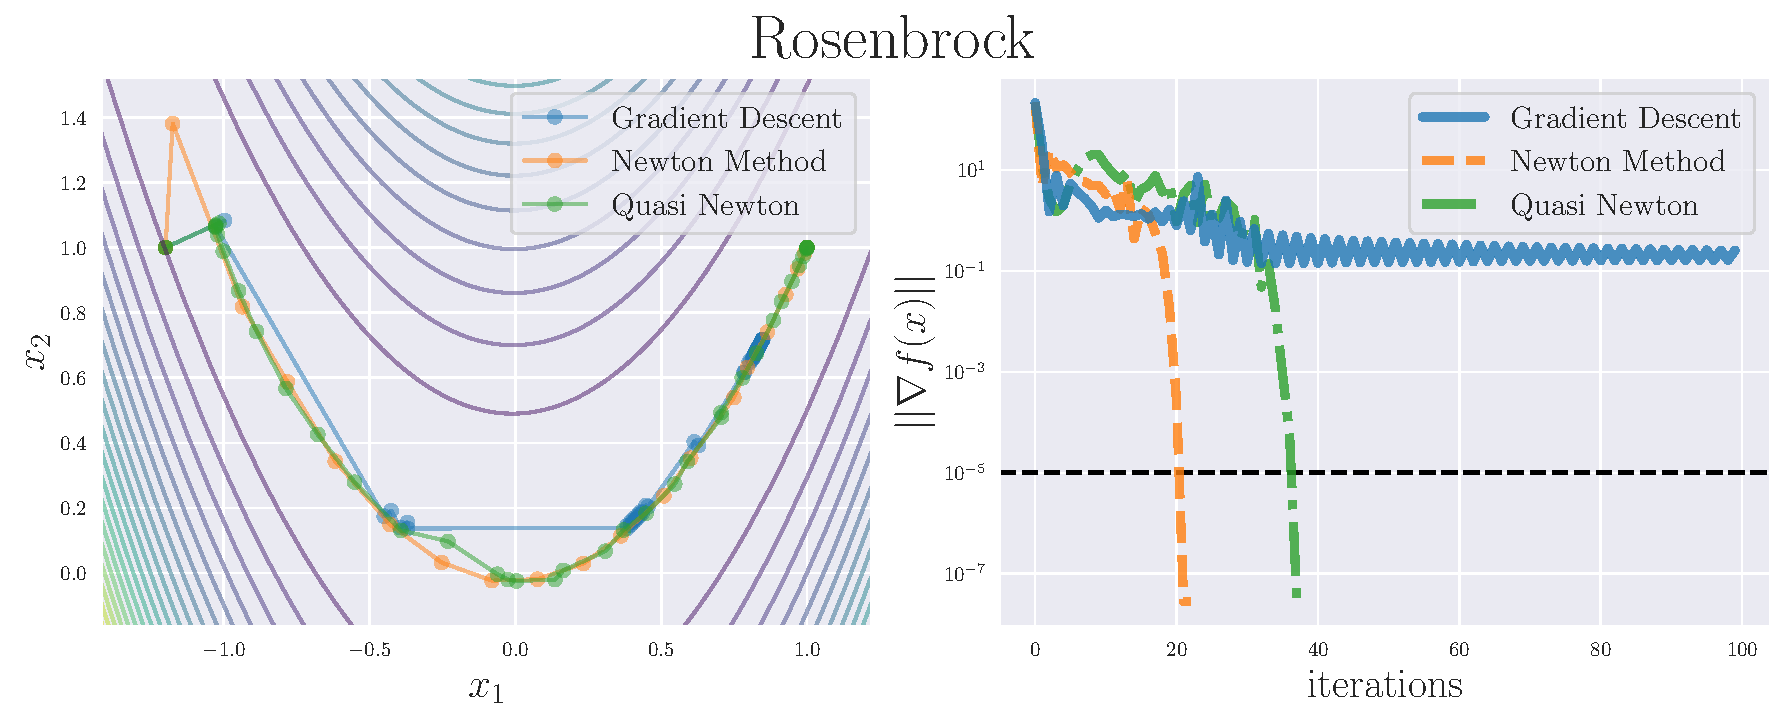
\includegraphics[width=\textwidth]{../imgs/quasi_newton/newton_vs_qs_vs_gd.pdf}
    \caption{
        \ifEn
            Comparison of Newton's method, quasi-Newton methods, and gradient descent.
        \else
            ニュートン法、準ニュートン法、勾配降下法の比較。
        \fi
    }
    \label{fig:newton_vs_qs_vs_gd}
\end{figure}

\ifEn
    Line search based quasi-Newton methods generate a sequence $\{ x_k \}_k$ that converges to the optimal solution $x^*$ as follows:
\else
    直線探索に基づく準ニュートン法では、最適解 $x^*$ に収束する列 $\{ x_k \}_k$ を次のように生成します。
\fi
\begin{equation*}
    x_{k+1} = x_k - \alpha_k B_k^{-1} \nabla f(x_k)
    = x_k - \alpha_k H_k \nabla f(x_k).
\end{equation*}
\ifEn
    Here, $\alpha_k > 0$ is the step size determined by line search, $B_k$ is an approximation of the Hessian matrix $\nabla^2 f(x_k)$ at the point $x_k$, and $H_k \coloneqq B_k^{-1}$ denotes its inverse. This update rule closely resembles that of Newton's method, which is why it is called a quasi-Newton method.
\else
    ここで $\alpha_k > 0$ は直線探索で定めるステップサイズであり、$B_k$ は点 $x_k$ におけるヘッセ行列 $\nabla^2 f(x_k)$ の近似です。$H_k \coloneqq B_k^{-1}$ はその逆行列を表します。この更新則はニュートン法の更新則と酷似しており、その故にこの手法は準ニュートン法と呼ばれています。
\fi

\ifEn
    The core of quasi-Newton methods lies in how to update $B_k$ at each iteration so that it approaches the true Hessian matrix.
    \Cref{fig:quasi_newton_overview} illustrates this concept. First, around the current point $x_k$, a quadratic approximation model of the objective function $f$ is constructed using $B_k$. Next, this quadratic model is minimized to obtain the next point $x_{k+1}$. After obtaining $x_{k+1}$, the approximation matrix $B_k$ is updated to $B_{k+1}$ using the gradient information at $x_k$ and $x_{k+1}$. This procedure is repeated until convergence, which constitutes the quasi-Newton method.
\else
    準ニュートン法の核心は、各反復で $B_k$ をどのように更新して真のヘッセ行列に近づけるかにあります。\Cref{fig:quasi_newton_overview} は準ニュートン法の概念図です。まず現在の点 $x_k$ の周りで、$B_k$ を用いて目的関数 $f$ の二次近似モデルを構成します。次にこの二次モデルを最小化して次の点 $x_{k+1}$ を得ます。$x_{k+1}$ を得た後、$x_k$ と $x_{k+1}$ における勾配情報を用いて近似行列 $B_k$ を $B_{k+1}$ に更新します。この手続きを収束するまで繰り返すことが準ニュートン法です。
\fi

\begin{figure}[t]
    \begin{minipage}{0.33\textwidth}
        \centering
        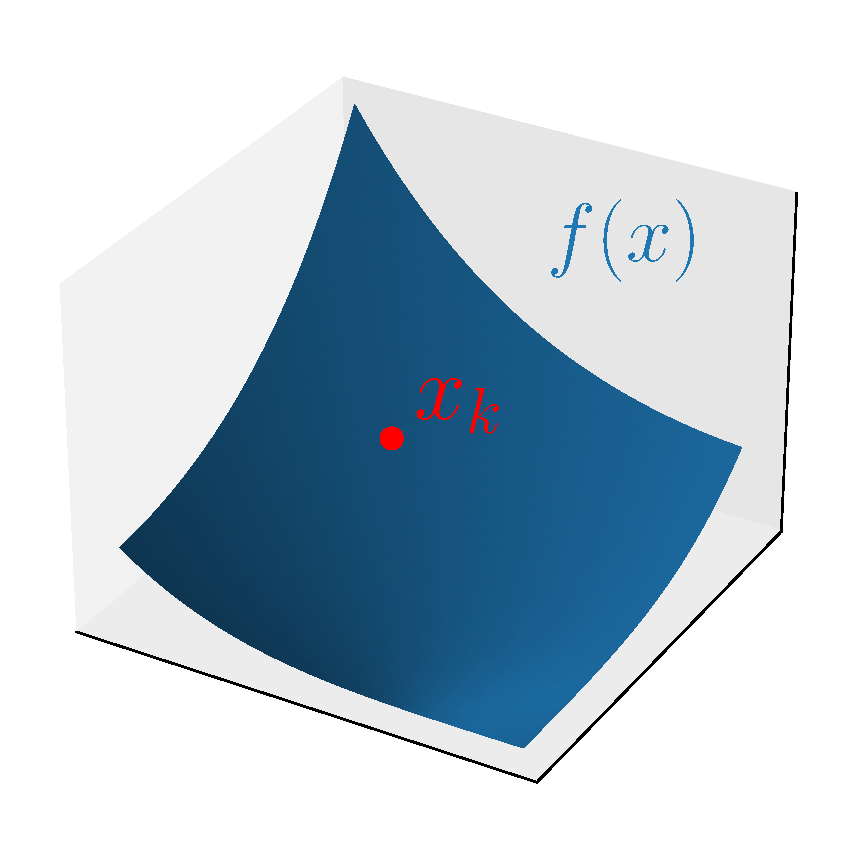
\includegraphics[width=\textwidth]{../imgs/quasi_newton/quasi_newton_1.pdf}
    \end{minipage}%
    \begin{minipage}{0.33\textwidth}
        \centering
        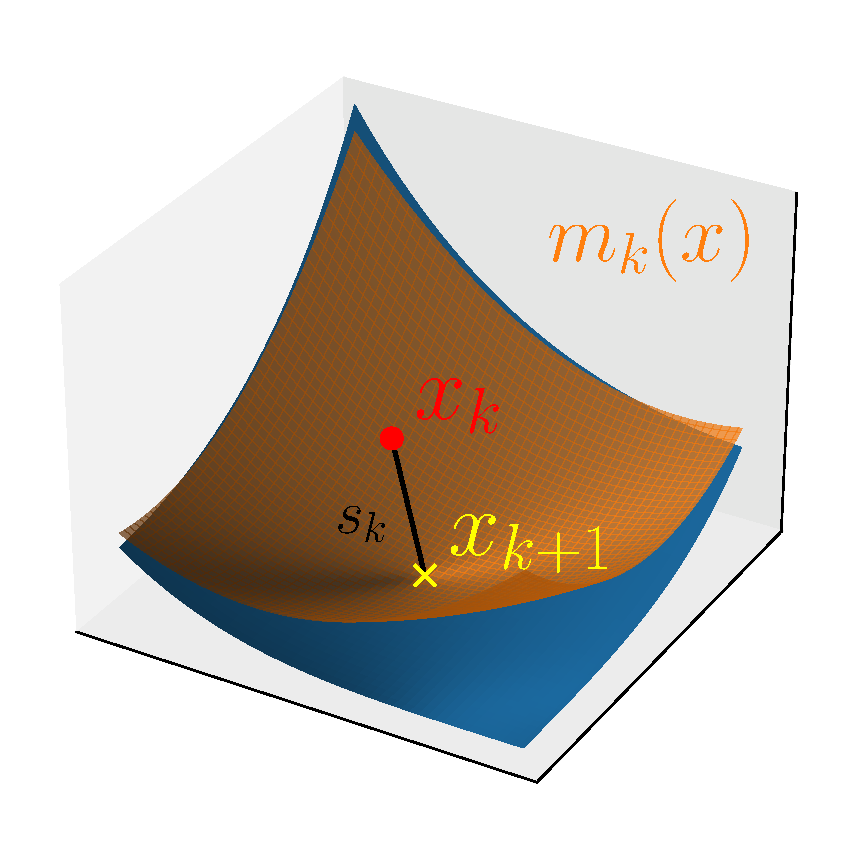
\includegraphics[width=\textwidth]{../imgs/quasi_newton/quasi_newton_2.pdf}
    \end{minipage}%
    \begin{minipage}{0.33\textwidth}
        \centering
        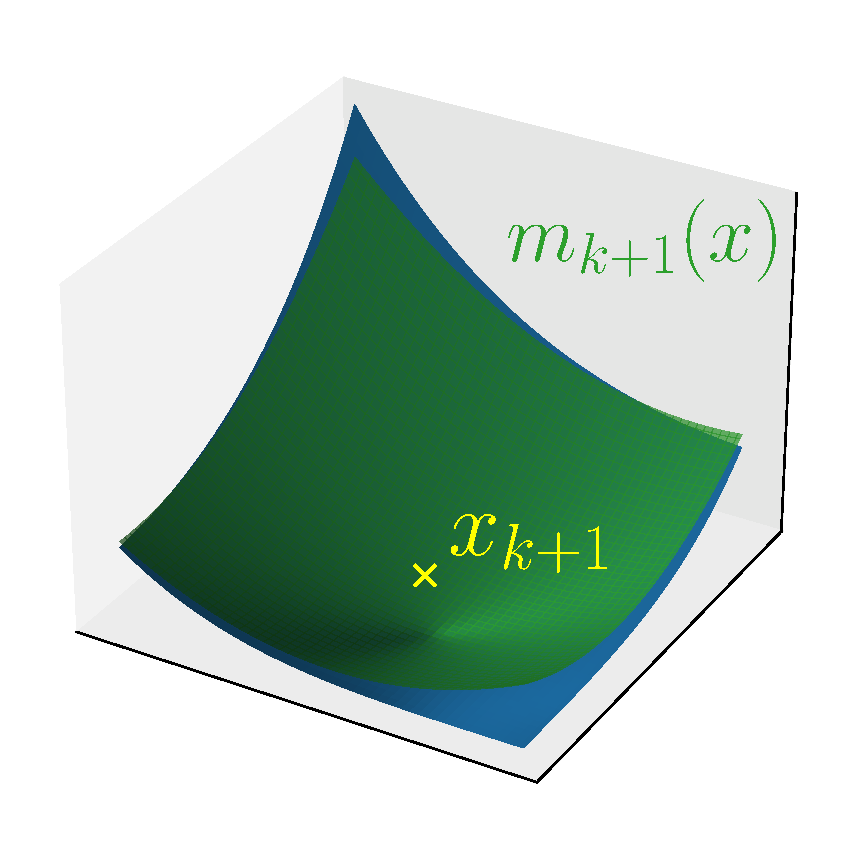
\includegraphics[width=\textwidth]{../imgs/quasi_newton/quasi_newton_3.pdf}
    \end{minipage}
    \caption{
        \ifEn
            Conceptual illustration of quasi-Newton methods.
            (1) Given the objective function $f$ (blue surface) and the current point $x_k$ (red point).
            (2) Move to the minimizer $x_{k+1}$ (yellow cross) of the quadratic model $m_k(x)$ (orange surface) constructed using the current approximate Hessian.
            (3) Update the quadratic model (green surface) and repeat this procedure.
        \else
            準ニュートン法の概念図。
            (1) 目的関数 $f$ (青い曲面) と現在点 $x_k$ (赤点) が与えられます。
            (2) 現在の近似ヘッセ行列によって得られる二次モデル $m_k(x)$ (橙色の曲面) を最小化し、その最小点 $x_{k+1}$ (黄色のバツ印) に移動します。
            (3) 二次モデルを更新し (緑色の曲面)、この操作を繰り返します。
        \fi
    }
    \label{fig:quasi_newton_overview}
\end{figure}

% QIITA_GIF (This is a placeholder for a GIF illustrating for qiita)

\ifEn
    \subsection{Secant Condition}
\else
    \subsection{セカント条件}
\fi

\ifEn
    Let $f\colon \mathbb{R}^n \to \mathbb{R}$ be of class $C^2$. Suppose that a symmetric matrix $B_k$ is given as an approximation of the Hessian matrix $\nabla^2 f(x_k)$. We consider updating the approximate Hessian to $B_{k+1}$ for the next point $x_{k+1}$. Although there are infinitely many possible candidates for such a matrix, it is natural to impose symmetry on $B_{k+1}$, since the true Hessian matrix is symmetric. For the current point $x_k$ and the next point $x_{k+1}$, we define the step and the gradient difference as follows:
\else
    関数 $f\colon \mathbb{R}^n \to \mathbb{R}$ を $C^2$ 級とします。対称行列 $B_k$ が点 $x_k$ におけるヘッセ行列 $\nabla^2 f(x_k)$ の近似として与えられたとき、次の点 $x_{k+1}$ における近似ヘッセ行列 $B_{k+1}$ への更新を考えます。このような行列の候補は無数に存在しますが、真のヘッセ行列が対称であることから、$B_{k+1}$ にも対称性を課すのが自然です。現在の点 $x_k$ と次の点 $x_{k+1}$ に対して、ステップと勾配差を次のように定義します。
\fi
\begin{equation*}
    s_k \coloneqq x_{k+1} - x_k, \qquad   y_k \coloneqq \nabla f(x_{k+1}) - \nabla f(x_k).
\end{equation*}
\ifEn
    In the following, we generally assume that $s_k \neq 0$ and $y_k^\top s_k \neq 0$.
    Note that the $s$ in $s_k$ stands for ``step.'' Since the new approximation is constructed around $x_{k+1}$, we approximate $\nabla f(x_k)$ using the Hessian matrix $\nabla^2 f(x_{k+1})$ and its approximation $B_{k+1}$ as follows:
\else
    以降では基本的に $s_k \neq 0$ かつ $y_k^\top s_k \neq 0$ とします。 なお、$s_k$ の $s$ は step を意味します。新しい近似は $x_{k+1}$ を中心に構築されるため、$\nabla f(x_k)$ をヘッセ行列 $\nabla^2 f(x_{k+1})$ およびその近似である $B_{k+1}$ を用いて次のように近似します。
\fi
\begin{align*}
    \nabla f(x_k) & \approx \nabla f(x_{k+1}) + \nabla^2 f(x_{k+1})(x_k - x_{k+1}) \\
                  & \approx \nabla f(x_{k+1}) + B_{k+1}(x_k - x_{k+1}).
\end{align*}
\ifEn
    Requiring the above approximation to hold as an equality yields
\else
    上の近似を等式として要求すると、次を得ます。
\fi
\begin{equation*}
    B_{k+1}(x_{k+1} - x_k) = \nabla f(x_{k+1}) - \nabla f(x_k).
\end{equation*}
\ifEn
    Equivalently, this can be rewritten as
\else
    あるいは同値に、
\fi
\begin{equation*}
    B_{k+1} s_k = y_k.
\end{equation*}
\ifEn
    This relation is called the secant condition or the quasi-Newton equation.
\else
    この関係はセカント条件、または準ニュートン方程式と呼ばれています。
\fi

\ifEn
    More precisely, the secant condition can also be justified as follows. Consider a quadratic approximation model around $x_{k+1}$:
\else
    より厳密には、セカント条件は次のようにも正当化できます。$x_{k+1}$ の周りの二次近似モデルを考えます。
\fi
\begin{equation*}
    m_{k+1}(x) = f(x_{k+1}) + \nabla f(x_{k+1})^\top (x - x_{k+1}) + \frac{1}{2} (x - x_{k+1})^\top B_{k+1} (x - x_{k+1}).
\end{equation*}
\ifEn
    By construction, regardless of $B_{k+1}$, this model satisfies
\else
    このモデルは構成上、$B_{k+1}$ によらず次を満たします。
\fi
\begin{equation*}
    \begin{cases}
        m_{k+1}(x_{k+1}) = f(x_{k+1}), \\
        \nabla m_{k+1}(x_{k+1}) = \nabla f(x_{k+1}).
    \end{cases}
\end{equation*}
\ifEn
    In addition, the secant condition ensures that the model satisfies
\else
    さらに、セカント条件により、このモデルは次も満たします。
\fi
\begin{align*}
    \nabla m_{k+1}(x_k) & = \nabla f(x_{k+1}) - B_{k+1} (x_{k+1} - x_k)             &  & (\text{definition of the model}) \\
                        & = \nabla f(x_{k+1}) - (\nabla f(x_{k+1}) - \nabla f(x_k)) &  & (\text{secant condition})        \\
                        & = \nabla f(x_k).
\end{align*}
\ifEn
    This implies that the secant condition ensures that the quadratic model $m_{k+1}(x)$ accurately reflects the known information at both $x_{k+1}$ and $x_k$, except for the previous function value $f(x_k)$.
\else
    これは、セカント条件により二次モデル $m_{k+1}(x)$ が、以前の関数値 $f(x_k)$ を除き、$x_{k+1}$ と $x_k$ の両方における既知の情報を正確に反映していることを意味しています。
\fi

\end{document}
